\documentclass[../main.tex]{subfiles}
\begin{document}

\chapter{Überblick}
\label{overview}
\pagenumbering{arabic}
  Virtualisierung entwickelte sich in den letzten Jahren zu einem allgegenwärtigen Thema in der \acrshort{IT}-Industrie. Unter ihr versteht man die Nachahmung und Abstraktion von physischen Resourcen, z.B. der \acrshort{CPU} oder des Speichers, die in einem virtuellen Kontext von Softwareprogrammen genutzt wird.

  Die Vorteile von Virtualisierung umfassen Hardwareunabhängigkeit, Verfügbarkeit, Isolierung und Sicherheit, welche die Erfolgsgrundlage der Virtualisierung in heutigen \gls{Cloud}-Infrastrukturen bilden \cite[S.1]{containerVirtPerformance}. Vor allem in Rechenzentren bieten sich Virtualisierungen an, um die Serverressourcen effizienter zu nutzen \cite[S.1]{dockerSec1}. Letztendlich haben es Virtualisierungen ermöglicht, Serverressourcen in der Form von \glspl{Cloud} wie z.B. den \emph{Amazon Web Services}\cite{amazonWebServices} und auf Basis eines Subskriptionsmodells nutzen zu können \cite[S.1]{dockerSec1}.

  Heutzutage existieren mehrere serverseitige Virtualisierungstechniken, wovon die Hypervisor-gestützen Methoden mit den etablierten Vertretern \emph{Xen}\cite{xen}, \emph{KVM}\cite{kvm}, \emph{VMware ESXi}\cite{vmwareESXi} und \emph{Hyper-V}\cite{hyperv} die meistverbreitesten sind \cite[S.2]{containerVirtPerformance}. Die alternative containerbasierte Virtualisierung erlebt mit dem Erfolg von Docker seit dessen Release im März 2013 einen Aufschwung \cite{githubDockerChangelog}. Wie die Google Trends in \fig \ref{fig:overview_googleTrends} zeigen, stieg das Interesse an Docker seit dessen Release kontinuierlich an, während das Suchwort \glqq{}virtualization\grqq{} im Jahr 2010 seinen Höhepunkt hatte und seitdem an Popularität verlor. Auch das Interesse an der Containertechnologie \emph{LXC}, aus der Docker entstand, bleibt weit hinter der von Docker zurück \cite{googleTrends}.

  \begin{figure}[h]
      \centering
      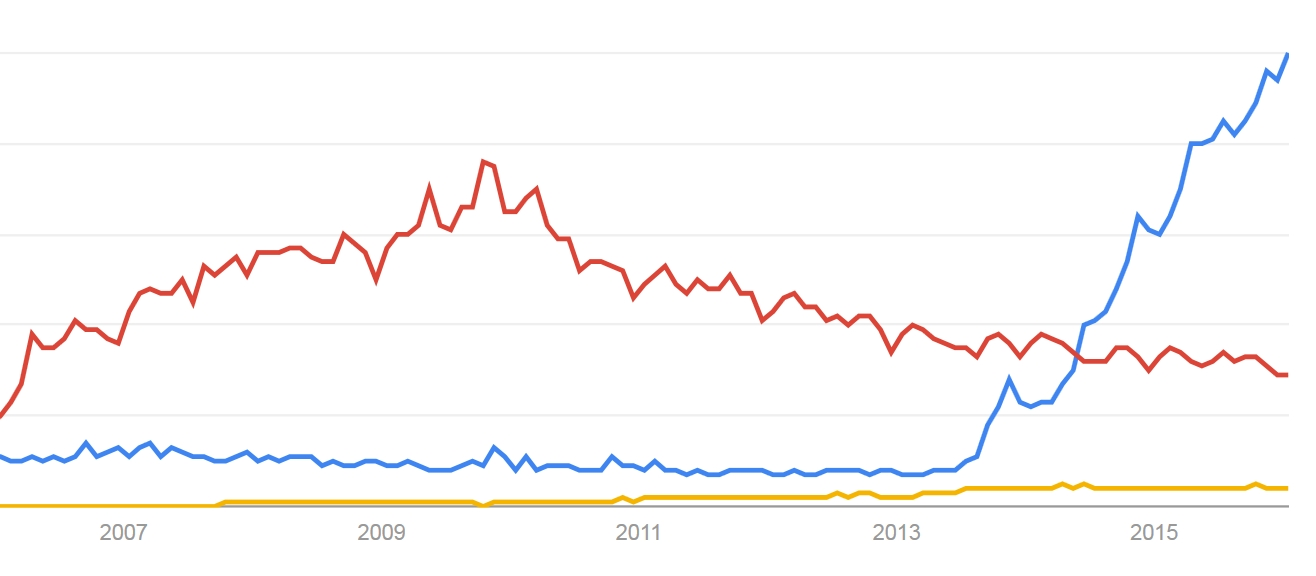
\includegraphics[width=1.0\textwidth]{./images/googletrend_dockerVirtualizationLXC.jpg}
      \caption{Google Trends der Suchbegriffe \glqq{}Virtualization\grqq{} (rot), \glqq{}Docker\grqq{} (blau) und \glqq{}LXC\grqq{} (gelb) von Januar 2006 bis Januar 2016\cite{googleTrends}.}
      \label{fig:overview_googleTrends}
  \end{figure}

  Obwohl das Konzept von Containern bereits im Jahr 2000 als \emph{Jails} in dem Betriebssystem \emph{FreeBSD} und seit 2004 als \emph{Zones} unter \emph{Solaris} verwendet wurde \cite{zonesReleasenotes}\cite{jailsReleasenotes}, gelang keiner dieser Technologien vor Docker der medienwirksame Durchbruch. Wie Docker den bis 2013 vorherrschenden Ruf von Containertechnologien, dass Container noch nicht ausgereift seien \cite[S.8]{containerVirtPerformance}, nachhaltig verändern konnte, ist in der Einführung zu Docker in Kapitel \ref{dockerIntro} beschreiben.

  Heute sind Container in vielen Szenarien, v.a. skalierbaren Infrastrukturen, trotz intrinsischer Sicherheitsschwächen gegenüber Hypervisor-gestützten Virtualisierungsarten beliebt. Vor allem \glspl{MultiTenantService} werden gerne mit Docker umgesetzt \cite[S.6]{dockerBook}\cite{dockerUnderstandingDocker}.

  % https://www.airpair.com/firebase/posts/yatodo-guide
  % https://www.airpair.com/docker/posts/8-proven-real-world-ways-to-use-docker#7-multi-tenancy

  \section{Struktur der Arbeit}
    Zu Beginn wird im Grundlagenkapitel \ref{introVirt} die Virtualisierung beschrieben. Dabei werden die zwei prominentesten Virtualisierungstechniken, Hypervisor-basierte (Sektion \ref{introVirtHypervisor}) und Container-basierte (Sektion \ref{introVirtContainer}) Virtualisierung, gegenübergestellt. In diesem Kapitel werden nur die für diese Arbeit relevante Techniken der Systemvirtualisierung beschrieben, also solche, in denen Funktionen von kompletten Betriebssystemen abstrahiert werden. Die Anwendungs-, Storage- oder Netzwerkvirtualisierung wird nicht behandelt. Anschließend werden die allgemeinen Sicherheitsziele in der \acrshort{IT} erklärt, auf die in der Untersuchung Bezug genommen wird. Abgeschlossen wird das Grundlagenkapitel mit einer Einführung in Docker, in der die Terminologie sowie Funktionsweise dieser Plattform erläutert wird.

    Die genannten Grundlagen sind sehr weitreichende Themengebiete. Um in den einleitenden Kapiteln nicht ausführlich zu werden, sind Eckdaten einiger am Rande auftretender Begriffe im angehängten Glossar zusammengefasst.

    Der Hauptteil untergliedert sich in mehrere Sicherheitsgebiete, in die die Arbeit eingeteilt ist:
    \begin{enumerate}
      \item \textbf{Sicherheitsfunktionen, die der Linux-Kernel anbietet} und teils obligatorisch von Docker eingesetzt werden. Darunter fallen Techniken zur Isolierung, Ressourcen- und Rechteverwaltung von Containern sowie Methoden, um das Hostsystem mit zusätzlichen Linux Sicherheitsfeatures abzusichern.
      \item \textbf{Sicherheit im Docker-Ökosystem}, also z.B.
        \begin{itemize}
          \item Integrität von Images
          \item Absicherung der Kommunikation zwischen dem Docker-Client und dem Docker-Host
          \item \glspl{BestPractice} im Umgang mit Docker-Komponenten sowie Sicherheitsrichtlinien.
          \item Verwendung von Third-Party Tools, wie \emph{Kubernetes} % TODO: Glossareintrag Third-Party
        \end{itemize}
      \item \textbf{Sicherheit von Docker in Cloud-Infrastrukturen}
        % TODO: Etwas mehr Details dazu, wenn klar ist was hier reinkommt.
    \end{enumerate}

    % TODO: Abgrenzung zu Netzwerkthemen, da das auf Netzebene passiert und Sicherheitsaspekte sind, die in jedem Netzwerk in Betracht gezogen werden müssen --> kein Bezug mehr zu Docker.

    Abgeschlossen wird die Arbeit mit einer Zusammenfassung und einem Ausblick auf die Zukunft von Docker und der containerbasierter Virtualisierung.

    In der Arbeit vorkommende Produkt-, Technologie- oder Unternehmensnamen sind durchgehend \emph{kursiv} gedruckt. Eine Ausnahme bildet Docker, in der die reguläre Schreibweise für die Plattform Docker vorgesehen ist, während die kursive Variante das Unternehmen \emph{Docker} meint.

\end{document}
